\documentclass[11pt]{article}

\usepackage[review]{acl}
\usepackage{times}
\usepackage{latexsym}
\usepackage[T1]{fontenc}
\usepackage[utf8]{inputenc}
\usepackage{microtype}
\usepackage{inconsolata}
\usepackage{graphicx}
\usepackage{amsmath}
\usepackage{booktabs}

\title{Mind the Cap: Output-Budget Regimes Change the Measured Multilingual Reasoning Gap}

\author{Anonymous}

\begin{document}
\maketitle

\begin{abstract}
Multilingual evaluations often report that models score higher when a problem is first translated into English, but this gap is usually measured at a single output-token cap. We test whether the native-vs-translate gap on MGSM (German, Thai, and Swahili) is a token-budget artifact, using Qwen3-8B and Llama-3.1-8B-Instruct. Budgets are prefixes of one stored 4096-token generation, so token-matched, FLORES-200-length-normalized, and dollar-matched comparisons all derive from a common ledger. Equation~(1) shows that the length-normalized contrast is exactly the NATIVE accuracy gain between the matched and the premium-scaled budget, so it must vanish once native accuracy saturates. At the prospectively frozen 1024-token budget, all six Holm-family Qwen tests fail to reject, because native-prefix accuracy is already flat in the budget at moderate levels; Llama likewise fails to reject, but its native accuracy is near floor and parseable answers often never appear. A retrospective sweep locates the budget-binding regime: tighter budgets change the measured gap by up to 38.9 points, and length normalization can reverse which strategy scores higher. COMET translation quality is high but uneven across model-language cells. Above score saturation, the residual difference is a strategy-performance gap, not an identified reasoning deficit. The same truncation channel prices a cost-ordered adaptation ladder: raising the serving budget and adding language-specific tokens both act only on traces the cap actually cuts, and a cross-fitted Thai vocabulary extension that lowers the token premium from 2.55 to 2.21 closes 0.00 points of the gap at the frozen budget while closing 4.9 points where 19\% of traces are still truncated. The output cap is therefore part of the evaluation estimand: multilingual evaluations should report accuracy across the budget regime, not at a single budget.
\end{abstract}

\section{Introduction}

A recurring finding in multilingual LLM evaluation is that models solve reasoning problems better when the problem is first translated into English than when they reason in the original language. This ``multilingual reasoning gap'' is usually measured at one generation length. Languages differ in how many tokens they need to express parallel content, and strategies differ in when they emit their answer. Under a hard output cap, both features interact with the cap in ways that can resemble a strategy-performance difference.

We ask a narrow, falsifiable question: is the native-vs-translate gap on MGSM a token-budget artifact? We operationalize a budget artifact as the change in that gap between a token-matched cap and a length-normalized, FLORES-200-premium-adjusted cap. If giving NATIVE its premium-scaled budget closes the gap, token matching contributed to the measured difference; if the gap persists, this particular correction does not explain it.

Our contribution is methodological:
\begin{enumerate}
    \item The measured contrast can depend strongly on the evaluation budget. We pair a prospectively frozen non-rejection at one budget with a retrospective sweep that locates the budget-binding regime.
    \item Under tight caps, length normalization can reverse which strategy looks better.
    \item Five ledger-computable audits---trace-language ID, COMET translation quality, parser robustness, decoder parity, and normalizer sensitivity---bound the interpretations the stored ledger supports.
    \item The same truncation channel prices a cost-ordered adaptation ladder: raising the serving budget and adding language-specific tokens act on the same traces, and a directly measured, cross-fitted vocabulary extension closes the gap only where the cap still truncates.
\end{enumerate}

Prompt language, reformulation, answer-format compliance, translation quality, and reasoning-trace language are confounded in this design. The object of inference is therefore strategy performance under controlled prefix budgets, not causal reasoning ability.

\section{Related work}
\label{sec:related}

This study connects multilingual chain-of-thought evaluation on MGSM \citep{mgsm} with work on test-time compute, output budgeting, and budget-forcing, including s1 \citep{s1budget}. Our length proxy follows the FLORES parallel-text lineage and NLLB's FLORES-200 benchmark \citep{flores101,nllb}, while the measurement checks use GlotLID \citep{glotlid} and COMET \citep{comet22}. Cross-lingual tokenization disparities make output length a language-specific computational cost \citep{ahia2023,petrov2023}; we study how a prefix budget changes a multilingual strategy contrast after language-length normalization. A common response to those disparities is to extend the vocabulary with target-language pieces and continue pretraining \citep{chinesellama,swallow}, optionally with a principled initialization for the new embeddings \citep{focus}; \S\ref{sec:ladder} prices that intervention against our estimand.

Inference-budget work likewise finds that truncating reasoning harms accuracy in model- and modality-dependent ways \citep{brokenchains}, while training models to recover answers from truncated traces could shrink the budget-binding regime \citep{trsd}. Multilingual studies find that English-pivot reasoning can improve accuracy yet drift off target \citep{mmath}, and identify input comprehension as a major loss source addressed by an English-intermediary pipeline \citep{ust}. Training-side methods further shrink native--pivot gaps to roughly 2--3.5\% under matched supervision \citep{layerswap} and produce cross-lingual self-distillation gains that grow with inference budget \citep{copsd}. Our contribution is orthogonal and evaluational: these methods should be measured under budget sweeps that reveal whether supervision, strategy, or answer-emission timing drives the reported gap.

\section{Design and estimands}
\label{sec:design}

\textbf{Data and strategies.} MGSM has 250 items per language in German (de), Thai (th), and Swahili (sw), three languages that span a wide range of FLORES-200 token premiums. We evaluate four strategies, also called arms: NATIVE (reason and answer in language \(L\)); TRANSLATE-ACT (translate the problem to English, then solve); PIVOT (English reasoning, answer in \(L\)); and CODE-SWITCHED (English scaffold). We draw \(k=8\) samples per item from Qwen3-8B \citep{qwen3} (confirmatory) and Llama-3.1-8B-Instruct \citep{llama3} (secondary, not a replication), for 48,000 stored generations.

\textbf{Prefix-defined budgets.} Each (item, sample) has one stored 4096-token generation. We call this store of generations, together with the scores of all their prefixes, the \emph{ledger}. Evaluating budget \(B\) means scoring the length-\(B\) prefix. This removes between-budget sampling noise but limits conclusions to prefix-defined evaluation; independently capped generations may differ. The retrospective regime sweep uses \(B \in \{64,128,192,256,384,512,768,1024\}\); 2048 and 4096 are added only for extended crossover and best-arm checks.

\textbf{Scoring.} We use strict prefix-only exact match on \texttt{\#\#\#\# <integer>} under intention to treat; truncated, non-integer, and non-compliant answers score 0. Each of the eight samples per item is scored independently at every budget---not by best-of-\(k\), pass@\(k\), or majority vote---and reported accuracy averages all item--sample cells; the item-clustered bootstrap resamples the 250 MGSM items while retaining all eight samples within each selected item.

\textbf{Estimand.} Let \(\operatorname{acc}_N\) and \(\operatorname{acc}_T\) denote NATIVE and TRANSLATE-ACT accuracy, let \(\operatorname{gap}(B)=\operatorname{acc}_T(B)-\operatorname{acc}_N(B)\), and let \(r_{m,L}\) be the FLORES-200 token premium of language \(L\) over English for model \(m\). Then
\begin{align}
\Delta_L(B)
&= [\operatorname{acc}_T(B)-\operatorname{acc}_N(B)] \notag\\
&\quad - [\operatorname{acc}_T(B)
          -\operatorname{acc}_N(\lfloor r_{m,L}B\rfloor)] \notag\\
&= \operatorname{acc}_N(\lfloor r_{m,L}B\rfloor)
   -\operatorname{acc}_N(B).
\end{align}

TRANSLATE-ACT cancels. What remains is simply how many more NATIVE answers become correct between the matched budget \(B\) and the premium-scaled budget \(\lfloor r_{m,L}B\rfloor\). We call a budget \emph{binding} when correct answer lines are still appearing inside that interval, and the \emph{budget-binding regime} is the range of \(B\) over which they are.

This identity has three direct consequences. First, \(\Delta_L(B)\) is a finite, discrete increment of the NATIVE accuracy curve, not a comparator interaction. Second, its peak location follows the NATIVE answer-emission distribution, while its height depends on the premium-scaled interval and the native curve inside it. Third, \(\Delta_L(B)\to0\) once NATIVE accuracy saturates, so a near-zero value above score saturation follows analytically from the estimand.

\textbf{Primary test.} The frozen evaluation budget is \(B^*=1024\), the largest \(B\in\{512,1024\}\) with every \(\lfloor r_{m,L}B\rfloor\le4096\). The confirmatory family contains six Holm-corrected Qwen tests: H1-existence, directional H1-SESOI (\(\Delta_L(B^*)>5\) points), H2 (a larger effect for Thai than German), and H3 (a dollar-matched strategy reversal) for each of the three languages. Inference uses an item-clustered paired bootstrap (10,000 resamples), a studentized sup-\(t\) maximum statistic, and a pre-specified \(1.3\times\) tail-conservatism factor; Appendix~\ref{app:stats} gives details. The exploratory two-sided equivalence statement below is separate. The analysis protocol was internally frozen before confirmatory scoring; this was not a public preregistration.

FLORES-200 premiums are Qwen de 1.56 / th 2.55 / sw 1.94 and Llama de 1.58 / th 2.19 / sw 1.93. For each model and language, \(r_{m,L}\) is the total-token ratio to parallel English over all 1,012 FLORES-200 devtest sentence pairs after NFC normalization, computed with that model's own tokenizer and a paired percentile bootstrap over sentence pairs.

\section{Regime-dependent results}
\label{sec:results}

\subsection{The frozen test yields no confirmatory support}
\label{subsec:frozen}

At \(B^*=1024\), \(\Delta_L(B^*)\) is near zero for every Qwen language, and all six Holm-family tests fail to reject (formal outcome \texttt{no\_confirmatory\_h1\_support}):
\begin{itemize}
    \item Qwen \(\Delta_L(B^*)\): de 0.00, th 0.15, sw 0.05 points. H1-existence raw \(p=0.060\) at Holm-local \(\alpha=0.0083\); H1-SESOI raw \(p=1.0\).
    \item Llama \(\Delta_L(B^*)\): de/th/sw all 0.00. This procedurally matched secondary analysis is outside the confirmatory family and also rejects nothing.
\end{itemize}

The two non-rejections have different descriptive causes. Qwen NATIVE accuracy plateaus at 79.0\% / 47.1\% / 33.7\% for de/th/sw; between 1024 and the Thai FLORES-scaled budget of 2611, only 3 of 2000 traces become newly correct. Llama NATIVE instead plateaus near floor at 13.6\% / 3.9\% / 29.0\%, alongside never-emission rates of 80.2\% / 93.2\% / 46.0\%. Qwen therefore reaches score saturation at moderate accuracy, whereas Llama de/th often never produces a parseable native answer. Neither pattern implies that all traces have terminated.

\subsection{Tight budgets expose a large, then vanishing, artifact}
\label{subsec:tight}

Table~\ref{tab:peak-accuracy} places the largest retrospective \(\Delta_L(B)\) inside the budget-binding regime (pointwise item-clustered bootstrap 95\% CIs).

\begin{table*}[t]
\centering
\small
\caption{Peak length-normalization effects, where \(\Delta_L(B)=\operatorname{acc}_N(\lfloor rB\rfloor)-\operatorname{acc}_N(B)\), together with values at the frozen budgets. Intervals are pointwise item-clustered bootstrap 95\% CIs.}
\label{tab:peak-accuracy}
\resizebox{\textwidth}{!}{%
\begin{tabular}{lrrrrrr}
\toprule
model/lang & peak \(\Delta_L(B)\) (pts) & peak \(B\) & NATIVE acc. at \(B\) & TRANSLATE-ACT acc. at \(B\) & \(\Delta_L(512)\) & \(\Delta_L(1024)\) \\
\midrule
Qwen de  & 34.2 [30.2, 38.3] & 192 & 16.10 & 22.60 & 2.25 & 0.00 \\
Qwen th  & 38.9 [34.7, 43.0] & 256 & 6.20  & 47.75 & 8.85 & 0.15 \\
Qwen sw  & 15.0 [12.4, 17.7] & 128 & 8.70  & 0.60  & 0.25 & 0.05 \\
Llama de & 8.4 [7.0, 9.9]    & 256 & 3.85  & 43.10 & 0.15 & 0.00 \\
Llama th & 2.3 [1.6, 3.1]    & 192 & 1.10  & 16.90 & 0.15 & 0.00 \\
Llama sw & 18.2 [15.9, 20.6] & 256 & 8.25  & 44.60 & 1.60 & 0.00 \\
\bottomrule
\end{tabular}
}
\end{table*}

The Qwen rows of Table~\ref{tab:peak-accuracy} contain three different kinds of peak. German gives the clearest two-arm comparison: at \(B=192\) both arms are well away from floor, and premium-scaling raises NATIVE by 34.2 points.

Thai has the largest peak, and also the largest premium: at \(B=256\), \(r=2.55\) gives a premium-scaled budget of 652, so \(\Delta_L(256)\) summarizes the gain across a 396-token interval rather than a contrast at equal output widths.

Swahili is weaker evidence. Its peak occurs where TRANSLATE-ACT scores only 0.60\%, so it shows a native-prefix rescue rather than a clean two-arm comparison away from floor. The same caution applies to the German crossover at \(B=128\) (\S\ref{subsec:crossover}).

Simultaneous max-\(|t|\) 95\% bands over the sweep keep every Qwen peak away from zero (de@192 [27.8, 40.6], th@256 [32.3, 45.4], sw@128 [10.7, 19.3]), and peak locations are stable in 89.6\%, 100.0\%, and 87.9\% of bootstrap replicates. At \(B^*\) the largest language-specific upper bound is 0.32 points for Qwen and 0.00 for Llama, below the exploratory \(\pm5\)-point equivalence margin.

\textbf{Normalizer sensitivity.} The behavioral trace-length ratio is smaller than the FLORES premium in all six model-language cells, with non-overlapping pointwise intervals (Appendix~\ref{app:ratio}). FLORES therefore consistently grants the larger premium.

Substituting the behavioral ratio would still produce a 5-point artifact in four of the six cells. The minimum evaluated premium that produces a 5-point artifact lies below the behavioral ratio for Qwen de (1.089 vs 1.467) and th (1.188 vs 2.038), and for Llama de (1.274 vs 1.432) and sw (1.253 vs 1.848). Qwen Swahili is the exception: its threshold of 1.254 sits above the behavioral ratio of 1.179, so the 5-point Swahili claim depends on a premium above that ratio, including the frozen FLORES token premium. Llama Thai never reaches 5 points, even at \(1.5\times\) FLORES.

These thresholds are grid-selected and conditional on the stored traces. The behavioral ratio is not a validated normalizer, because it compares traces that differ in content, correctness, and stopping behavior.

Figure~\ref{fig:native-curves} plots the Qwen NATIVE curves and marks both accuracy endpoints of each peak premium interval.

\begin{figure*}[t]
\centering
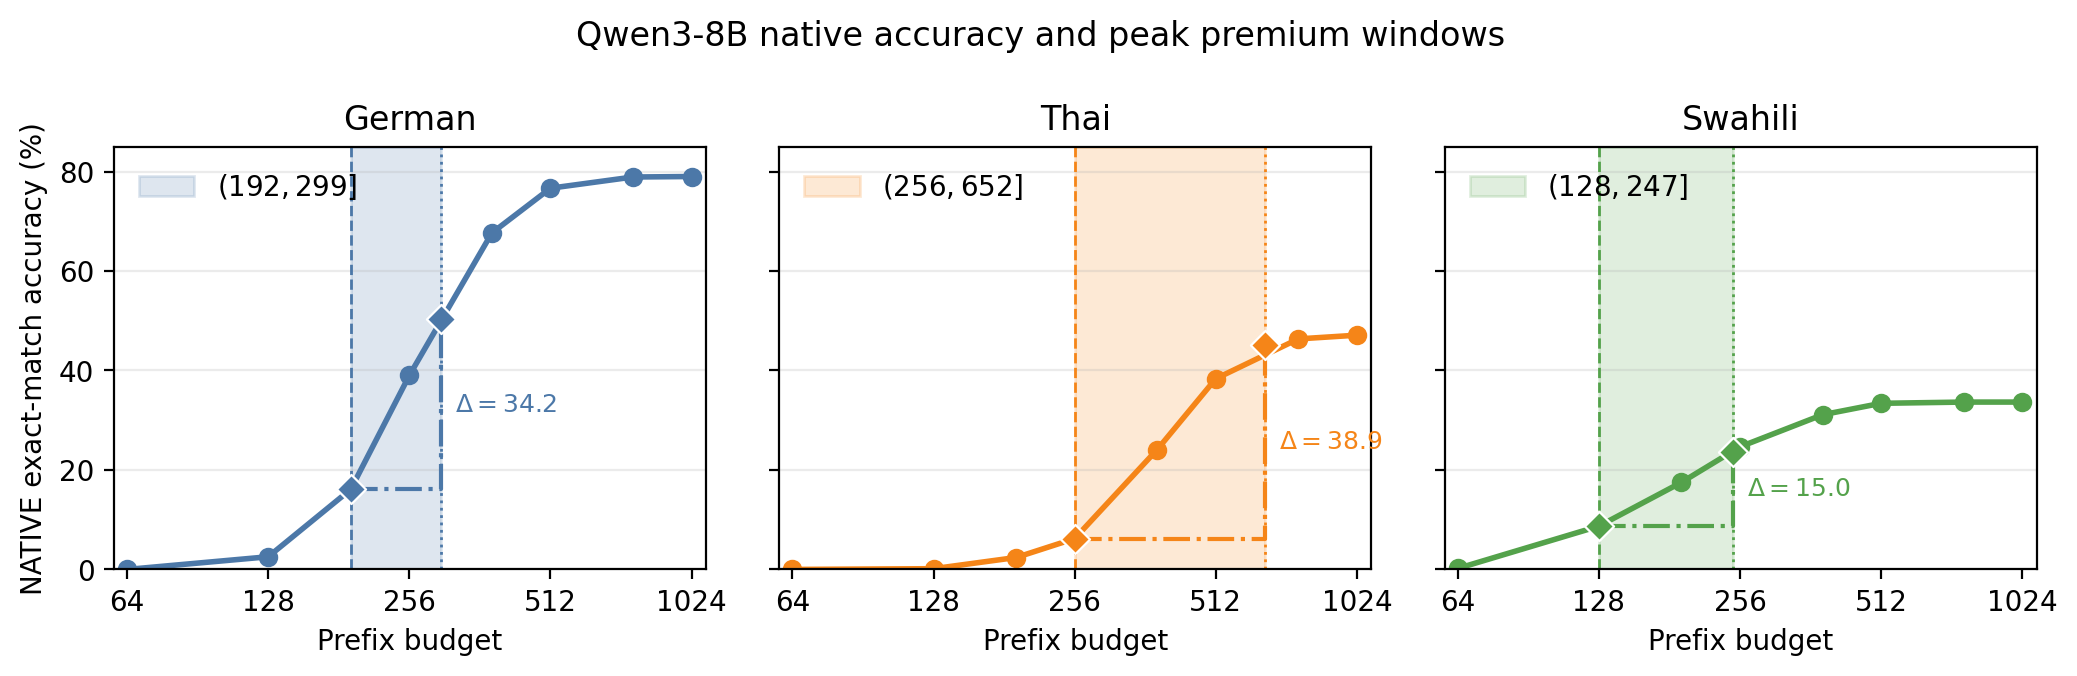
\includegraphics[width=\textwidth]{native_curves.png}
\caption{Qwen NATIVE accuracy by budget. Shaded intervals mark each language's peak normalization interval \((B_{\mathrm{peak}},\lfloor rB_{\mathrm{peak}}\rfloor]\); the vertical gain between the endpoint markers equals the peak \(\Delta_L(B)\).}
\label{fig:native-curves}
\end{figure*}

\subsection{Tight caps can reverse strategy rankings}
\label{subsec:crossover}

Table~\ref{tab:emission-timing} shows that Qwen crossover strength follows the left tail of answer-emission timing more closely than the medians.

\begin{table*}[t]
\centering
\small
\caption{Qwen answer-emission timing and observed strategy crossovers. \(E\) is the token position at which a parseable answer is emitted; p10 is its 10th percentile.}
\label{tab:emission-timing}
\resizebox{\textwidth}{!}{%
\begin{tabular}{lrrrrl}
\toprule
lang & NATIVE median \(E\) & TRANSLATE-ACT median \(E\) & NATIVE p10 \(E\) & TRANSLATE-ACT p10 \(E\) & observed crossover \\
\midrule
sw & 206 & 262 & 96  & 170.7 & strongest: NATIVE leads at 64/128/192 \\
de & 270 & 247 & 160 & 158   & marginal: NATIVE leads at 128 \\
th & 377 & 250 & 236 & 165   & none \\
\bottomrule
\end{tabular}
}
\end{table*}

TRANSLATE-ACT's median emission is earlier than NATIVE's in German and Thai. The p10 ordering is timing-consistent with the crossover: Swahili has a 74.7-token NATIVE early-tail advantage and the strongest native lead; German differs by only 2 tokens and has a narrow lead; Thai NATIVE is 71 tokens later and never leads. These grid-resolved emission summaries do not isolate translation-segment length or establish mediation.

At \(B=128\), Qwen German NATIVE scores 2.55\% versus 1.15\% for TRANSLATE-ACT; Swahili NATIVE leads with bootstrap probability 1.00 at 128 and 192 (transition [192,256]), while German leads with probability 0.958 at 128 (transition [128,192]). Thai has no native lead, and no Llama language crosses because native accuracy remains near floor. The Qwen Swahili crossover also comes from a degenerate heavy-tail cell: NATIVE output-length p90 is 4096 and 25.1\% never emit a parseable answer. The frozen H3 test did not detect these reversals because it examined only the looser pre-specified budgets.

\section{Measurement audits}
\label{sec:audits}

We report five ledger audits and one diagnostic. Trace-language ID, COMET, parser robustness, and decoder parity appear below; normalizer sensitivity appears in \S\ref{subsec:tight}. The verbosity/failure-tail decomposition is a diagnostic, not a sixth audit.

\textbf{Trace-language ID (automated GlotLID).} Automated labels support the main NATIVE vs TRANSLATE-ACT contrast. Determinate NATIVE traces are classified in \(L\) at Qwen de 92.1\% / sw 94.1\% / th 99.4\%, and at approximately 100\% for all Llama languages; TRANSLATE-ACT post-delimiter reasoning is 98.4--99.9\% English.

Three caveats apply. First, the initial \texttt{swh}-only mapping failed the frozen native:sw agreement criterion (75\% \(<\) 90\%). We then adopted the Swahili macrolanguage remap (\texttt{swh}+\texttt{swc}, with \texttt{swc} denoting Congo Swahili), which raised Qwen native-Swahili compliance from 85.8\% to 94.1\% and the validation cell to 90.00\% (18/20); because this remap was adopted after inspecting the failure, we report it as a post-hoc analytic decision. Unrelated neighboring Bantu labels remain outside Swahili. Second, an independent blind LLM adjudication of 240 Qwen traces agrees at 96.7\% overall and at least 90\% in every cell, but it is preliminary and the frozen human validation remains outstanding. Third, PIVOT and CODE-SWITCHED violate their English instruction in 9 of 12 cells, so they remain outside the main comparison.

\textbf{COMET translation quality.} Reference-based COMET is generally high but nonuniform (Table~\ref{tab:comet}): German is strongest for both models (0.877 Qwen, 0.872 Llama), Qwen Swahili is lowest at 0.749, and Llama Thai has a weak lower tail (p10 0.325). At the six prespecified peak budgets, an exploratory per-cell analysis finds weak and inconsistent COMET--correctness-gain associations (Spearman \(\rho=-0.143\) to \(0.280\), five positive, only one with \(|\rho|\ge0.20\); Table~\ref{tab:comet-gain}), so the tight-budget TRANSLATE-ACT advantage is not well explained by translation quality. Translation quality remains part of the strategy bundle; these scores are descriptive and never condition accuracy.

\textbf{Parser robustness.} In NATIVE peak cells, prefix-only rescued-correct traces are at most 0.35\% and value-unstable traces at most 0.30\%. Within the \((B,\lfloor rB\rfloor]\) intervals, 96.8--100\% of native gains are genuinely terminated, and requiring a terminated answer line changes every peak by at most 0.2 points. The tight-budget effect is therefore late answer emission rather than a prefix-parser artifact.

\textbf{Decoder parity.} A stratified 2,520-prefix audit finds 37.9\% raw exact-string agreement between local and vLLM decoding but 100\% agreement after production special-token normalization, including 100\% parsed-answer and correctness agreement. All raw divergences are cosmetic special-token markup.

\textbf{Verbosity/failure-tail diagnostic.} Qwen Swahili NATIVE has a heavy tail: 10.6\% hit the 4096 cap and 25.1\% never emit a parseable answer. This mixes truncation, non-integer or multiple answers, and format noncompliance, cautioning against interpreting native accuracy as pure reasoning ability.

\section{Implications for adaptation}
\label{sec:ladder}

A natural response to a measured multilingual gap is a cost-ordered ladder of
fixes: raise the serving budget, then change the prompting strategy, then add
language-specific tokens to the tokenizer, and finetune only if all three fail.
Two of those rungs act through the same channel, and our ledger lets us price
them.

\textbf{Both token-count rungs act only by relieving truncation.} A larger cap
and a cheaper tokenizer both change one thing: how much of the trace the model
is allowed to finish. Where the trace already fits, neither can change an
answer. This is the same channel Equation~(1) describes---writing \(\rho\) for
the factor by which an extension shortens target-language text, a NATIVE-only
payoff of \(\operatorname{acc}_N(\lfloor\rho B\rfloor)-\operatorname{acc}_N(B)\)
has exactly the form of Equation~(1) with \(\rho\) in place of \(r_{m,L}\). We
use that only as motivation, not as a result: compression is not uniform across
traces, and a deployed extension changes both arms, so we measure the effect
directly rather than substituting \(\rho\) into the identity.

\textbf{Measurement, not extrapolation.} We built genuinely extended Qwen
tokenizers---base vocabulary and merge list untouched, new byte-level merges
learned on target-language traces and appended so that base merges retain
priority---and then measured what they buy under a cap. Each stored trace is
retokenized with the extended tokenizer, its first \(B\) extended token ids are
decoded, and that text is scored with the same strict parser used throughout
the paper; the baseline is the identical computation with the base tokenizer.
No uniform compression factor is applied. Training text is the NATIVE arm only:
the PIVOT and CODE-SWITCHED arms are substantially English in several cells
(Swahili PIVOT is 90.1\% English, \S\ref{sec:audits}) and would not train a
language-specific vocabulary. Extensions are cross-fitted over two disjoint
halves of the item set, so no evaluated item contributed a merge, and the
extension size is fixed in advance by a rule that never consults
accuracy---the largest extension each fold's corpus admits. This yields roughly
3.4k, 6.7k and 3.1k new tokens for de/th/sw, which cut the FLORES-200 devtest
premium from 1.559 to 1.531, from 2.551 to 2.207, and from 1.936 to 1.846,
while changing the aggregate English devtest token count by less than
\(0.02\%\) (Appendix~\ref{app:vocab}).

The extension is applied to both arms, so \(G_3\) reflects one deployment
change rather than a NATIVE-only advantage. Because TRANSLATE-ACT traces are
largely English, a target-language extension barely compresses them; their
gains are correspondingly small, which is a property of the intervention rather
than an artifact of the design.

This is a token-count-only counterfactual, not a prediction about a retrained
model. It holds the emitted text fixed and changes only what that text costs. A
real extension must also learn embeddings for the new tokens
\citep{chinesellama,swallow,focus}, which is itself a training procedure, and a
model whose tokenizer changed would follow a different trajectory.

\begin{table*}[t]
\centering
\small
\caption{Adaptation triage for Qwen. \(G\) is the NATIVE deficit against
TRANSLATE-ACT at the deployed cap \(B\); \(G(4096)\) is the deficit at the
largest stored prefix; \(G_3\) is the deficit after a cross-fitted
language-specific vocabulary extension applied to both arms at the original
cap. ``NAT.\ trunc.'' is the share of NATIVE traces longer than \(B\); ``NAT.\
gain'' is \(\operatorname{acc}_N(4096)-\operatorname{acc}_N(B)\), the NATIVE
accuracy actually recovered by extending the prefix to the largest one stored.
It is observed on this ledger, not a general ceiling: 4096 still binds, and it
does not bound gap closure, which also depends on TRANSLATE-ACT. Gap closure carries item-clustered bootstrap
95\% CIs, conditional on the two fitted tokenizers. The prompting rung is not
priced: the comparator TRANSLATE-ACT \emph{is} that rung, so it closes \(G\) by
construction.}
\label{tab:ladder}
\begin{tabular}{lrrrrrrl}
\toprule
lang & \(B\) & NAT.\ trunc. & NAT.\ gain & \(G\) & \(G(4096)\) & \(G_3\) (vocab) & gap closed by vocab [95\% CI] \\
\midrule
de & 128  & 97.1\% & 76.45 & \(-1.40\)  & \(+9.40\)  & \(-2.30\)  & \(+0.90\) [\(-0.05\), 1.85] \\
de & 256  & 52.1\% & 40.00 & \(+10.25\) & \(+9.40\)  & \(+9.05\)  & \(+1.20\) [\(-0.25\), 2.65] \\
de & 512  & 3.9\%  & 2.35  & \(+10.95\) & \(+9.40\)  & \(+10.45\) & \(+0.50\) [0.05, 1.10] \\
de & 1024 & 0.2\%  & 0.00  & \(+9.35\)  & \(+9.40\)  & \(+9.35\)  & \(+0.00\) [0.00, 0.00] \\
\midrule
th & 128  & 99.9\% & 47.10 & \(+0.75\)  & \(+40.60\) & \(-0.10\)  & \(+0.85\) [0.20, 1.65] \\
th & 256  & 84.7\% & 41.05 & \(+41.55\) & \(+40.60\) & \(+38.15\) & \(+3.40\) [1.90, 5.00] \\
th & 512  & 18.9\% & 8.90  & \(+48.40\) & \(+40.60\) & \(+43.50\) & \(+4.90\) [3.65, 6.20] \\
th & 1024 & 0.7\%  & 0.15  & \(+40.75\) & \(+40.60\) & \(+40.75\) & \(+0.00\) [0.00, 0.00] \\
\midrule
sw & 128  & 81.5\% & 25.05 & \(-8.10\)  & \(+23.30\) & \(-9.40\)  & \(+1.30\) [0.75, 1.90] \\
sw & 256  & 42.6\% & 9.00  & \(+5.00\)  & \(+23.30\) & \(+4.35\)  & \(+0.65\) [\(-0.20\), 1.55] \\
sw & 512  & 15.3\% & 0.35  & \(+22.75\) & \(+23.30\) & \(+22.80\) & \(-0.05\) [\(-0.25\), 0.15] \\
sw & 1024 & 11.6\% & 0.10  & \(+23.40\) & \(+23.30\) & \(+23.35\) & \(+0.05\) [0.00, 0.15] \\
\bottomrule
\end{tabular}
\end{table*}

Table~\ref{tab:ladder} prices the ladder, and three patterns cut against the
monotone \(G>G_1>G_2>G_3\) expectation.

First, \emph{more budget need not shrink the gap}. At \(B=128\) the measured
deficit is negative in German and Swahili and near zero in Thai, because
TRANSLATE-ACT has not finished its translation preamble
(\S\ref{subsec:crossover}); at the largest stored prefix Swahili moves from
\(G=-8.10\) to \(+23.30\). These cells sit near the accuracy floor---both arms
are below 10\% at \(B=128\)---so this is an exploratory sign instability rather
than a calibrated estimate of harm. It is nonetheless enough to show that a gap
measured under a tight cap can carry the wrong sign.

Second, \emph{vocabulary extension captures only a fraction of what a larger
cap would}. The informative comparison is not the truncated share but
\(\operatorname{acc}_N(4096)-\operatorname{acc}_N(B)\), the NATIVE accuracy a
longer prefix actually recovers: truncated traces that were never going to be
scored correct cannot be rescued by any token-count intervention. Against that
quantity, the extension's own NATIVE gain is 3.45 of 40.00 points for German at
\(B=256\) (9\%) and 5.20 of 41.05 for Thai (13\%), rising to 5.05 of 8.90 for
Thai at \(B=512\) (57\%). Its largest gap closure anywhere in our data is 4.90
points, and its largest NATIVE gain is 5.20. Where the longer prefix recovers
nothing the extension does too: at \(B=1024\) the NATIVE gain to 4096 is 0.00 /
0.15 / 0.10 points and closure is \(0.00/0.00/0.05\). German at \(B=256\) and
Swahili at \(B=256\) and \(512\) have intervals that include zero.

The Swahili rows show why the truncated share alone is misleading. At
\(B=1024\), 11.6\% of NATIVE traces exceed the cap, but 211 of those 232 traces
run to the 4096-token generation cap without stopping, only 23 are parseable
even from the full stored trace, and only two become correct by 4096. The
NATIVE gain to 4096 is therefore 0.10 points, of which the extension recovers
0.05. The
cell is not evidence that extension is weak against real truncation; it is a
cell with almost nothing left to recover within the ledger, and reporting
truncation without the realized gain would have obscured that.

Third, \emph{the residual gap is the whole gap}. At the largest stored prefix,
9.4 / 40.6 / 23.3 points remain for de/th/sw. We cannot report the prompting
rung as a validated intervention, because adopting TRANSLATE-ACT closes \(G\)
by definition; its standalone value would have to be established against a
different comparator.

Two cautions constrain how far this generalizes. Our ledger caps generation at
4096 tokens, so \(G(4096)\) is the gap at the largest prefix we stored, not a
demonstrated non-binding regime; 10.55\% of Swahili NATIVE generations reach
that cap without stopping. And the scale of the intervention is modest by
construction: cutting the Thai premium from 2.551 to 2.207 is 13.5\% fewer
tokens for the same text, equivalently 15.6\% more text under a fixed cap,
against the four- to thirty-two-fold increases available by raising the cap
itself.

The practical guidance is therefore narrow. Before paying for either
token-count rung, measure the realized gain directly: extend the cap on a
sample and see how much accuracy the longer prefixes actually recover. Where
that gain is small, neither rung is likely to pay, however many traces the cap
truncates---though this is dispositive only if the extended cap is itself
non-binding, which ours is not. Where the gain is large, our data do not
support a general ordering: raising the cap dominates
for \emph{native accuracy}---40.00 against 3.45 points for German at
\(B=256\)---but not necessarily for the \emph{gap}, because a larger cap lifts
TRANSLATE-ACT too, which is why German gap closure is 1.20 points from
extension against 0.85 from raising the cap, and why Swahili's gap widens from
5.00 to 23.30. Vocabulary extension may also reduce decoding steps, though we
did not measure net serving cost or latency, and a larger embedding and output
projection work against the saving. We did not test the finetuning rung, the
prompting rung is confounded with our comparator, and this is one model family
on one benchmark, so this is a triage heuristic derived from our estimand, not
a validated adaptation method.

\section{Scope and implications}
\label{sec:scope}

In these stored-prefix MGSM evaluations, multilingual exact-match comparisons are regime-dependent: length normalization has large descriptive effects while answer emission binds, and negligible effects after score saturation. The prospectively frozen non-rejection at \(B^*=1024\) is a negative boundary condition; the retrospective sweep locates where the sensitivity actually occurs.

At the larger evaluated budgets the residual native-vs-translate difference is large (Qwen Thai about +41 points, Llama Thai about +69), but it is a strategy-performance gap. Prompt language, reformulation, format compliance, translation quality, and reasoning language remain confounded.

Calling this residual ``not an identified reasoning deficit'' states what our design can identify, not that execution effects are absent: complementary diagnostics find genuine target-language reasoning-execution failures even with English inputs \citep{datg}.

\textbf{Limitations.} (i) Scores come from prefixes of one long decode, not independently hard-capped decodes; decoder parity establishes scoring parity, not trajectory parity, and hard caps could elicit different trajectories, so the prefix-based magnitudes are an upper-relevance bound pending independently capped replication. The tight-budget result is retrospective and exploratory. (ii) vLLM repeat generation was only 46\% bitwise deterministic, preserving the stored-ledger estimand but weakening reproducibility and shared-seed interpretation. (iii) Scope is MGSM, three languages, and two 8B models. (iv) The frozen human GlotLID validation remains outstanding, despite the preliminary blind LLM agreement. (v) The frozen same-content trace-premium validation was not performed; the behavioral ratio in Appendix~\ref{app:ratio} does not substitute for it. (vi) Calibration is only approximately nominal (corrected type-I 0.00917 vs 0.00833 target); the \(1.3\times\) factor is a family-wide safeguard, not a verified family-wise calibration. (vii) The vocabulary-extension results in \S\ref{sec:ladder} are a token-count-only counterfactual: prefixes are rescored under an extended tokenizer while the emitted text is held fixed, so they do not predict a retrained model, whose trajectory would differ and whose new embeddings must themselves be learned. They cover Qwen alone because the extension is tokenizer-specific; the extensions are trained on MGSM reasoning traces rather than general text, so the compression we observe is a property of this corpus and not a bound on what is achievable; appending merges preserves base-merge priority but not every English segmentation; and we did not measure net serving cost or latency, which a larger embedding matrix would partly offset. The bootstrap resamples items while holding the two cross-fitted tokenizers fixed, so the intervals are conditional on that draw and do not propagate the uncertainty of learning the merges; the fold split is fixed rather than randomized, and we did not run repeated splits. Both arms in Table~\ref{tab:ladder} are scored by retokenizing the stored text rather than by replaying stored token ids; the two agree on 59{,}998 of 60{,}000 sample-budget comparisons and differ by at most 0.10 accuracy points in any reported cell. \(G(4096)\) is the gap at the largest stored prefix, not a demonstrated non-binding regime, since 4096 is the generation cap and 10.55\% of Swahili NATIVE generations reach it. The emission percentiles quoted in \S\ref{sec:ladder} are computed among emitting traces only, covering neither the 1.95--25.1\% that never emit nor the upper tenth that emit late. The \(B=128\) sign reversals sit near the accuracy floor.

Future work should test prompt interventions that elicit earlier answer emission---which would shrink NATIVE's budget-binding regime---and extend the protocol beyond MGSM numeric exact match to longer-form and non-numeric tasks.

\textbf{Data and code availability.} The full ledger of stored generations and all analysis code will be released.

\textbf{Takeaway.} When comparing language strategies under a token cap, treat the cap as an independent variable rather than a background constant. Report accuracy across a budget sweep with a length-normalized comparison, mark the region in which answer emission binds, and do not let a single budget carry the claim.

\bibliography{custom}

\appendix

\section{Accuracy-curve summary}
\label{app:curves}

The complete curves use \(B\in\{64,128,192,256,384,512,768,1024\}\). Qwen NATIVE accuracy rises from 0.0/0.0/0.2\% at \(B=64\) to 79.0/47.1/33.7\% at \(B=1024\) for de/th/sw; Llama NATIVE rises from 0.0/0.0/0.0\% to 13.6/3.9/29.0\%. The Qwen curves climb sharply through the peak intervals in Figure~\ref{fig:native-curves} and then flatten, whereas the Llama de/th curves remain near floor. The supplementary material reports every model--language--arm value at all eight budgets.

\section{Best-English-arm}
\label{app:bestarm}

Reselecting the empirically best English arm inside each bootstrap replicate reproduces the preselected TRANSLATE-ACT gap closely (Qwen Thai about 41 points, Llama Thai about 69; uplift over TRANSLATE-ACT is near zero in most cells).

\section{Trace-length ratio (not a normalizer)}
\label{app:ratio}

The ratio of median NATIVE output tokens to median TRANSLATE-ACT post-delimiter English-reasoning tokens is Qwen de 1.47 / th 2.04 / sw 1.18. Subtracting the FLORES premium gives a negative difference in all six cells, with non-overlapping pointwise intervals: Qwen de \(-0.092\) [\(-0.144\), \(-0.028\)], th \(-0.513\) [\(-0.588\), \(-0.440\)], sw \(-0.757\) [\(-0.824\), \(-0.685\)]; Llama de \(-0.149\) [\(-0.193\), \(-0.099\)], th \(-0.427\) [\(-0.488\), \(-0.365\)], sw \(-0.083\) [\(-0.129\), \(-0.021\)]. This ratio compares behaviorally different traces and cannot validate or replace FLORES.

\section{Statistical machinery and the six-test family}
\label{app:stats}

The Qwen confirmatory family contains exactly six raw p-values, corrected by Holm at family level \(\alpha=0.05\): H1-existence tests whether any language has \(\Delta_L>0\); H1-SESOI separately tests whether any has \(\Delta_L>5\) points; H2 tests the directional ordered contrast \(\Delta_{\mathrm{th}}-\Delta_{\mathrm{de}}>0\); and H3-de, H3-th, and H3-sw each test for a dollar-matched strategy reversal, requiring a significantly positive NATIVE-minus-TRANSLATE-ACT contrast at one common-support budget and a significantly negative contrast at another. Each H3 p-value is the maximum of the multiplicity-controlled positive- and negative-side p-values, an intersection-union test.

Inference resamples the 250 parallel MGSM items as clusters, retaining all languages, arms, and eight samples within each selected item, for 10,000 paired bootstrap resamples. Studentized sup-\(t\) maxima provide simultaneous bounds over languages for H1 and over budgets for H3; H2 uses the corresponding one-sided studentized bootstrap contrast. Because calibration with 250 discrete item clusters found mild anti-conservatism in the extreme \(\alpha/6\) tail, every raw confirmatory p-value is multiplied by the pre-specified 1.3 tail-conservatism factor (capped at 1), equivalently testing at \(\alpha/1.3\), before Holm correction.

\section{TRANSLATE-ACT translation quality (COMET, descriptive)}

Reference-based \texttt{Unbabel/wmt22-comet-da}; one stored full trace per item (sample 0); delimiter-missing traces excluded from this denominator only; pointwise 95\% item-bootstrap CIs (10,000 resamples).

\begin{table*}[t]
\centering
\small
\caption{Reference-based COMET translation quality for TRANSLATE-ACT. Intervals are pointwise 95\% item-bootstrap CIs.}
\label{tab:comet}
\resizebox{\textwidth}{!}{%
\begin{tabular}{llrrrrrrr}
\toprule
Model & Lang & n & Missing delimiter & COMET mean & median & p10 & p90 & 95\% CI \\
\midrule
Qwen  & de & 250 & 0.0\% & 0.877 & 0.878 & 0.834 & 0.921 & [0.872, 0.881] \\
Qwen  & th & 249 & 0.4\% & 0.858 & 0.866 & 0.810 & 0.907 & [0.851, 0.865] \\
Qwen  & sw & 250 & 0.0\% & 0.749 & 0.772 & 0.580 & 0.867 & [0.734, 0.763] \\
Llama & de & 249 & 0.4\% & 0.872 & 0.874 & 0.826 & 0.915 & [0.868, 0.877] \\
Llama & th & 244 & 2.4\% & 0.783 & 0.850 & 0.325 & 0.895 & [0.759, 0.805] \\
Llama & sw & 240 & 4.0\% & 0.798 & 0.825 & 0.703 & 0.888 & [0.783, 0.811] \\
\bottomrule
\end{tabular}
}
\end{table*}

These scores are descriptive only and never condition, gate, or reweight accuracy.

\begin{table}[t]
\centering
\small
\caption{Exploratory COMET association with correctness gain at each prespecified peak token budget, using sample 0. Intervals are pointwise bootstrap 95\% CIs.}
\label{tab:comet-gain}
\resizebox{\columnwidth}{!}{%
\begin{tabular}{llrrr}
\toprule
Model & Lang & Peak \(B\) & \(n\) & Spearman \(\rho\) [95\% CI] \\
\midrule
Qwen  & de & 192 & 250 & 0.015 [\(-0.112\), 0.139] \\
Qwen  & th & 256 & 249 & 0.146 [0.019, 0.269] \\
Qwen  & sw & 128 & 250 & \(-0.143\) [\(-0.269\), \(-0.004\)] \\
Llama & de & 256 & 249 & 0.280 [0.155, 0.399] \\
Llama & th & 192 & 244 & 0.009 [\(-0.129\), 0.146] \\
Llama & sw & 256 & 240 & 0.074 [\(-0.051\), 0.203] \\
\bottomrule
\end{tabular}
}
\end{table}

\section{Vocabulary-extension measurement}
\label{app:vocab}

We extend the Qwen3-8B byte-level BPE tokenizer without touching the base
vocabulary or merge list. New merges are learned on target-language traces and
appended below every base merge, so base merges retain priority. Training text
comes from the NATIVE arm only, because the PIVOT and CODE-SWITCHED arms are
substantially English in several Qwen cells (\S\ref{sec:audits}). Extensions
are cross-fitted over two disjoint halves of the 250 MGSM items: each extension
is trained on the NATIVE traces of the items it is \emph{not} evaluated on, so
no evaluated item contributed a merge to the tokenizer that scores it, for
either arm. The base pipeline reproduces the frozen premiums exactly (1.5589 /
2.5508 / 1.9363).

The English control compares aggregate English devtest token counts before and
after extension. It bounds the aggregate cost below \(0.02\%\), but appending
merges guarantees only that base merges retain priority; it does not guarantee
that every English string segments identically, and a small number do change.

\begin{table}[t]
\centering
\small
\caption{Qwen vocabulary extension, per cross-fitting fold. \(r\) is the frozen
FLORES-200 premium and \(r'\) is the premium under the extended tokenizer. The
English control is the aggregate English devtest token count relative to the
base tokenizer. These are the extensions used in Table~\ref{tab:ladder}.}
\label{tab:vocab}
\begin{tabular}{llrrrr}
\toprule
Lang & Fold & New tokens & \(r\) & \(r'\) & English \\
\midrule
de & 0 & 3{,}470 & 1.559 & 1.531 & 0.99996 \\
de & 1 & 3{,}343 & 1.559 & 1.532 & 0.99996 \\
th & 0 & 6{,}798 & 2.551 & 2.195 & 1.00000 \\
th & 1 & 6{,}577 & 2.551 & 2.218 & 1.00000 \\
sw & 0 & 3{,}173 & 1.936 & 1.865 & 0.99993 \\
sw & 1 & 3{,}054 & 1.936 & 1.826 & 0.99986 \\
\bottomrule
\end{tabular}
\end{table}

Extension sizes are limited by our corpora, which are MGSM reasoning traces
rather than general target-language text; a production-scale extension trained
on a broader corpus would plausibly compress more, but we cannot bound that
from these data, so we report the compression observed under this corpus rather
than a lower bound on what is achievable.

Accuracy in Table~\ref{tab:ladder} does not use \(\rho\) as a multiplier. Each
stored trace is retokenized with the extended tokenizer, its first \(B\)
extended token ids are decoded, and the resulting text is scored with the
strict parser; the baseline runs the same code with the base tokenizer.
Decoding token ids, rather than slicing the source string at a token offset,
matters because byte-level tokens can split a code point, so an offset slice
would occasionally admit slightly more than \(B\) tokens. Scoring generated
text rather than stored token ids is a reimplementation of the scorer used
elsewhere in the paper, so we verified it against that scorer on all six Qwen
cells at five budgets: the two paths agree on 59{,}998 of 60{,}000
sample-budget comparisons, the two exceptions being Swahili NATIVE traces whose
text does not round-trip to its stored token ids. Every column of
Table~\ref{tab:ladder} is produced by the retokenization path alone, so the
reported closure is exactly \(G-G_3\). No model weights are trained.

\end{document}
